% Made up for the tikra benchmark.
\definecolor{indigo}{RGB}{60,20,110}
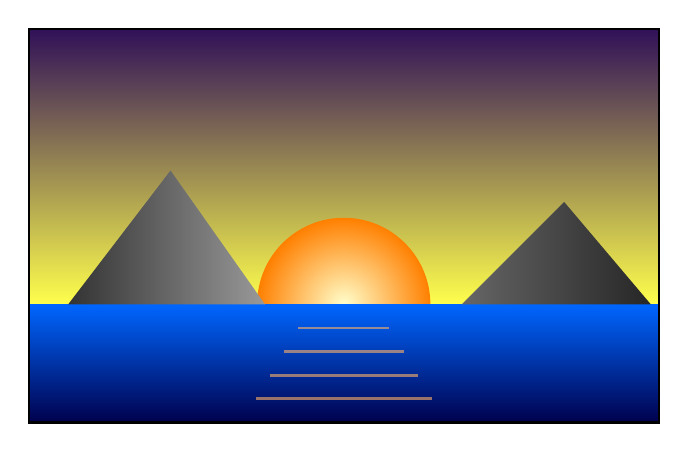
\begin{tikzpicture}
  \shade[top color=indigo!80!black, middle color=orange!90, bottom color=yellow!70] (0,1.5) rectangle (8,5);
  \shade[inner color=yellow!20, outer color=orange] (4,1.5) circle (1.1);
  \shade[top color=blue!60!cyan, bottom color=blue!30!black] (0,0) rectangle (8,1.5);
  \foreach \y in {0.3,0.6,...,1.3}
    \draw[orange!60, line width=1pt, opacity=0.6] (4-1.3+\y*0.6,\y) -- (4+1.3-\y*0.6,\y);
  \shade[left color=black!80, right color=black!40] (0.5,1.5) -- (1.8,3.2) -- (3,1.5) -- cycle;
  \shade[left color=black!60, right color=black!85] (5.5,1.5) -- (6.8,2.8) -- (7.9,1.5) -- cycle;
  \draw[thick] (0,0) rectangle (8,5);
\end{tikzpicture}
